\chapter{API REST}
\label{capapi}

Este capitulo esta destinado a los desarrolladores que deseen interactuar con el VirtShell API, para realizar aprovisionamientos autom'aticos desde cualquier plataforma de desarrollo. El VirtShell API es un API REST que provee accesso a los objetos en el VirtShell Server, esto incluye los hosts, imagenes, archivos, templates, aprovisionadores y usuarios. Por medio del API podr'a crear ambientes, m'aquinas virtuales y contenedores personalizados, realizar configuraciones y administrar los recursos f'isicos y virtuales de manera program'atica. 

\section{Formato de entrada y salida}
El API solo soporta el formato json para intercambio de informaci'on. Cualquier solicitud que no se encuentre en formato json resultara en un error con codigo 406 (Content Not Acceptable Error).

\section{Codigos de error}
Aqui se presenta una lista de codigos de error que pueden resultar de una petici'on al API en cualquier recurso.

\begin{itemize}
\item \textbf{400 Bad Request} La solicitud no pudo ser procesada con 'exito porque el URI no era v'alido. El cuerpo de la respuesta contendr'a una raz'on del fracaso de la petici'on. Esta respuesta indica error permanente.

\item \textbf{403 Forbidden} La solicitud no pudo ser procesada con 'exito porque la identidad del usuario no tiene acceso suficiente para procesar la solicitud. Esta respuesta indica error permanente.

\item \textbf{406 Content Not Acceptable} Un recurso genera este error de acuerdo al tipo de cabeceras enviadas en la petici'on. Esta respuesta indica un error permanete e indica un formato de salida no soportado. La respuesta de este tipo de error no contiene un contenido debido a la inhabilidad del servidor para generar una respuesta en el formato solicitado.

\item \textbf{404 Not Found} La solicitud no pudo ser procesada con 'exito porque la solicitud no era v'alida. Lo m'as probable es que no se encontró la url. Esta respuesta indica error permanente.

\item \textbf{500 Server Error} La solicitud no pudo ser procesada debido a que el servidor encontr'o una condici'on inesperada que le impidi'o cumplir con la petici'on.

\item \textbf{501 Not Implemented} La solicitud no se pudo completar porque el servidor o bien no reconoce el m'etodo de petici'on o el recurso solicitado no existe.

\end{itemize}

Los errores que no sean de codigo 406 (Content Not Acceptable) contienen una respuesta en formato json, que contiene un breve mensaje explicado el error con m'as detalle. Por ejemplo, una consulta POST /virtshell/api/v1/hosts, con un cuerpo vacio, dar'ia lugar a la siguiente respuesta:

\vspace{1cm}
\begin{lstlisting}[style=json]
HTTP/1.1 400 Bad Request
Content-Type: application/json

{"error": "Missing input for create instance"}
\end{lstlisting}

\section{API Resources}

\subsection{Hosts}
Representan las m'aquinas f'isicas; un host es un anfitrion de m'aquinas virtuales o contenedores. Los metodos soportados son:

\begin{center}
 \begin{tabular}{| l | l | l | l |}
 \hline
  \rowcolor{blueapi}
  \textbf{Acci'on} & \textbf{Metodo HTTP} & \textbf{Solicitud HTTP} & \textbf{Descripci'on} \\ [0.5ex] 
  \hline\hline
  get & GET & /hosts/id & Gets one host by ID. \\
  \hline
  list & GET & /hosts & Retrieves the list of hosts. \\
  \hline  
  create & POST & /hosts/ & Inserts a new host configuration. \\
  \hline
  delete & DELETE & /hosts/id & Deletes an existing host. \\
  \hline  
  update & PUT & /hosts/id & Updates an existing host. \\ [1ex] 
  \hline
\end{tabular}
\end{center}

\vspace{1cm}
Representaci'on del recurso de un host:
\vspace{1cm}

\begin{lstlisting}[style=json]
{
  "uuid": string,
  "name": string,
  "os": string,
  "memory": string,
  "capacity": string,
  "enabled": string,
  "type":string,
  "local_ipv4": string,
  "local_ipv6": string,
  "public_ipv4": string,
  "public_ipv6": string,
  "instances": [ instance_resource],
  "created":["at": number, "by": number]
}
\end{lstlisting}

Ejemplo:

\medskip
\begin{lstlisting}[style=json]
{
  "uuid": "ab8076c0-db91-11e2-82ce-0002a5d5c51b",
  "name": "host-01-pdn",
  "os": "Ubuntu_12.04_3.5.0-23.x86_64",
  "memory": "16GB",
  "capacity": "120GB",
  "enabled": "true|false",
  "type":"StorageOptimized|GeneralPurpose|HighPerformance",
  "local_ipv4": "15.54.88.19",
  "local_ipv6": "ff06:0:0:0:0:0:0:c3",
  "public_ipv4": "10.54.88.19",
  "public_ipv6": "yt06:0:0:0:0:0:0:c3",
  "instances": [
    ... instances resource is here
  ],
  "created":["at":"timestamp", "by":1234]
}
\end{lstlisting}

\subsection{Ejemplos de peticiones HTTP}

\subsubsection{Crear un nuevo host - POST /virtshell/api/v1/hosts}

\begin{lstlisting}[style=json]
curl -sv -X POST \
  -H 'accept: application/json' \
    -H 'X-VirtShell-Authorization: UserId:Signature' \
  -d '{"name": "host-01-pdn",
       "os": "Ubuntu_12.04_3.5.0-23.x86_64",
       "memory": "16GB",
       "capacity": "120GB",
       "enabled": "true",
       "type" : "GeneralPurpose",
       "local_ipv4": "15.54.88.19",
         "local_ipv6": "ff06:0:0:0:0:0:0:c3",
       "public_ipv4": "10.54.88.19",
       "public_ipv6": "yt06:0:0:0:0:0:0:c3"}' \
   'http://localhost:8080/virtshell/api/v1/hosts'
\end{lstlisting}

\vspace{1cm}
Respuesta:
\vspace{1cm}

\begin{lstlisting}[style=json]
HTTP/1.1 200 OK
Content-Type: application/json
{ "create": "success" }
\end{lstlisting}

\subsubsection{Obtener un host- GET /virtshell/api/v1/hosts/:id}

\begin{lstlisting}[style=json]
curl -sv -H 'accept: application/json' 
     -H 'X-VirtShell-Authorization: UserId:Signature' \ 
     'http://localhost:8080/api/virtshell/v1/hosts?id=ab8076c0-db91-11e2-82ce-0002a5d5c51b'
\end{lstlisting}

\vspace{1cm}
Respuesta:
\vspace{1cm}

\begin{lstlisting}[style=json]
HTTP/1.1 200 OK
Content-Type: application/json
{
  "uuid": "ab8076c0-db91-11e2-82ce-0002a5d5c51b",
  "name": "host-01-pdn",
  "os": "Ubuntu_12.04_3.5.0-23.x86_64",
  "memory": "16GB",
  "capacity": "120GB",
  "enabled": "true",
  "type" : "StorageOptimized",
  "local_ipv4": "15.54.88.19",
  "local_ipv6": "ff06:0:0:0:0:0:0:c3",
  "public_ipv4": "10.54.88.19",
  "public_ipv6": "yt06:0:0:0:0:0:0:c3",
  "instances": [
    {
      "name": "name1",
      "id": "72C05559-0590-4DA6-BE56-28AB36CB669C"
    },
    {
      "name": "name2",
      "id": "17173587-C4E9-4369-9C43-FCBF5E075973"
    }
  ],
  "created":["at":"20130625105211", "by":10]
}
\end{lstlisting}

\subsubsection{Obtener todos los host - GET /virtshell/api/v1/hosts}

\begin{lstlisting}[style=json]
curl -sv -H 'accept: application/json' 
     -H 'X-VirtShell-Authorization: UserId:Signature' \ 
     'http://localhost:8080/api/virtshell/v1/hosts'
\end{lstlisting}

\vspace{1cm}
Respuesta:
\vspace{1cm}

\begin{lstlisting}[style=json]
HTTP/1.1 200 OK
Content-Type: application/json
{
  "hosts": [
    {
      "uuid": "ab8076c0-db91-11e2-82ce-0002a5d5c51b",
      "name": "host-01-pdn",
      "os": "Ubuntu_12.04_3.5.0-23.x86_64",
      "memory": "16GB",
      "capacity": "120GB",
      "enabled": "true",
      "type" : "StorageOptimized",
      "local_ipv4": "15.54.88.19",
      "local_ipv6": "ff06:0:0:0:0:0:0:c3",
      "public_ipv4": "10.54.88.19",
      "public_ipv6": "yt06:0:0:0:0:0:0:c3",
      "instances": [
        {
          "name": "name1",
          "id": "72C05559-0590-4DA6-BE56-28AB36CB669C"
        },
        {
          "name": "name2",
          "id": "17173587-C4E9-4369-9C43-FCBF5E075973"
        }
      ],
      "created":["at":"20130625105211", "by":10]
    },
    {
      "uuid": "ab8076c0-db91-11e2-82ce-0002a5d5c51b",
      "name": "host-01-pdn",
      "os": "Ubuntu_12.04_3.5.0-23.x86_64",
      "memory": "16GB",
      "capacity": "120GB",
      "enabled": "true",
      "type" : "GeneralPurpose",
      "local_ipv4": "15.54.88.19",
      "local_ipv6": "ff06:0:0:0:0:0:0:c3",
      "public_ipv4": "10.54.88.19",
      "public_ipv6": "yt06:0:0:0:0:0:0:c3",
      "instances": [
        {
          "name": "name3",
          "id": "DE11CC9A-482F-4033-A7F8-503EE449DD0A"
        },
        {
          "name": "name4",
          "id": "17173587-C4E9-4369-9C43-FCBF5E075973"
        },    
      ],
      "created":["at":"20130625105211", "by":10]
    }
  ]
}   
\end{lstlisting}

\subsubsection{Actualizar un host - PUT /virtshell/api/v1/hosts/:id}

\begin{lstlisting}[style=json]
curl -sv -X PUT \
  -H 'accept: application/json' \
    -H 'X-VirtShell-Authorization: UserId:Signature' \
  -d '{"memory": "24GB",
     "capacity": "750GB"}' \
   'http://localhost:8080/api/virtshell/v1/hosts?id=ab8076c0-db91-11e2-82ce-0002a5d5c51b'
\end{lstlisting}

\vspace{1cm}
Respuesta:
\vspace{1cm}

\begin{lstlisting}[style=json]
HTTP/1.1 200 OK
Content-Type: application/json

{ "update": "success" }
\end{lstlisting}

\subsubsection{Eliminar un host - DELETE /virtshell/api/v1/hosts/:id}

\begin{lstlisting}[style=json]
curl -sv -X DELETE \
   -H 'accept: application/json' \
   -H 'X-VirtShell-Authorization: UserId:Signature' \
   'http://localhost:8080/api/virtshell/v1/hosts?id=ab8076c0-db91-11e2-82ce-0002a5d5c51b'
\end{lstlisting}

\vspace{1cm}
Respuesta:
\vspace{1cm}

\begin{lstlisting}[style=json]
HTTP/1.1 200 OK
Content-Type: application/json
```
```json
{ "delete": "success" }
\end{lstlisting}

\subsection{Files}
Representan toda clase de archivos que se requieran para crear o aprovisionar m'aquinas virtuales o contenedores. Los metodos soportados son:

\begin{center}
 \begin{tabular}{| l | l | l | l |}
 \hline
  \rowcolor{blueapi}
  \textbf{Acci'on} & \textbf{Metodo HTTP} & \textbf{Solicitud HTTP} & \textbf{Descripci'on} \\ [0.5ex] 
  \hline\hline
  get & GET & /files/id & Gets one file by ID. \\
  \hline
  create & POST & /files/ & upload a new file. \\
  \hline
  delete & DELETE & /files/id & Deletes an existing file. \\
  \hline  
  update & PUT & /files/id & Updates an existing file. \\ [1ex]  
  \hline
\end{tabular}
\end{center}

\vspace{1cm}
Representaci'on del recurso de un archivo:
\vspace{1cm}

\begin{lstlisting}[style=json]
{
  "uuid": "ab8076c0-db91-11e2-82ce-0002a5d5c51b",
  "name": "file_name.extension",
  "folder_name" : "folder_name",
  "download_url": "https://<host>:<port>/api/virtshell/v1/files/folder_name/file.txt",
  "created":["at":"timestamp", "by":user_id]
}
\end{lstlisting}

Ejemplo:

\medskip
\begin{lstlisting}[style=json]
{
  "uuid": "ab8076c0-db91-11e2-82ce-0002a5d5c51b",
  "name": "ubuntu_seed_14-04.tex",
  "folder_name" : "ubuntu_seeds",
  "download_url": "https://<host>:<port>/api/virtshell/v1/files/ubuntu_seeds/ubuntu_seed_14-04.tex",
  "created": ["at":"20130625105211", "by":10]
}
\end{lstlisting}

\subsubsection{Ejemplos de peticiones HTTP}

\paragraph{Subir un nuevo archivo - POST /virtshell/api/v1/images} ~\\

\begin{lstlisting}[style=json]
curl -X POST \
  -H 'accept: application/json' \
  -H 'X-VirtShell-Authorization: UserId:Signature' \
  -H "Content-Type: multipart/form-data" \
  -F "file_data=@/path/to/file/seed_file.txt;filename=seed_file_ubuntu-14_04.txt" \
  -F "folder_name=ubuntu_seeds" \
  'http://<host>:<port>/api/virtshell/v1/files'
\end{lstlisting}

\vspace{1cm}
Respuesta:
\vspace{1cm}

\begin{lstlisting}[style=json]
HTTP/1.1 200 OK
Content-Type: application/json
{ 
  "create": "success",
  "location": "http://<host>:<port>/api/virtshell/v1/files/ubuntu_seeds/seed_file_ubuntu-14_04.txt" 
}
\end{lstlisting}

\paragraph{Obtener un archivo - GET /virtshell/api/v1/files/:id} ~\\

Para descargar un archivo, primero recibira la url apropiada que viene en la metadata provista por la url. Luego podra descargarlo usando la url.

\begin{lstlisting}[style=json]
curl -sv -H 'accept: application/json' 
     -H 'X-VirtShell-Authorization: UserId:Signature' \ 
     'http://<host>:<port>/api/virtshell/v1/files/?id=ab8076c0-db91-11e2-82ce-0002a5d5c51b'
\end{lstlisting}

\vspace{1cm}
Respuesta:
\vspace{1cm}

\begin{lstlisting}[style=json]
HTTP/1.1 200 OK
Content-Type: application/json
{
  "uuid": "ab8076c0-db91-11e2-82ce-0002a5d5c51b",
  "name": "file_name.extension",
  "folder_name" : "folder_name",
  "download_url": "http://<host>:<port>/api/virtshell/v1/files/ubuntu_seeds/seed_file_ubuntu-14_04.txt",
  "created":["at":"timestamp", "by":user_id] 
}
\end{lstlisting}

\paragraph{Actualizar un archivo - PUT /virtshell/api/v1/files/:id} ~\\

\begin{lstlisting}[style=json]
curl -sv -X PUT \
  -H 'accept: application/json' \
  -H 'X-VirtShell-Authorization: UserId:Signature' \
  -H "Content-Type: multipart/form-data" \
  -F "file_data=@/path/to/file/seed_file.txt;filename=seed_file_ubuntu-14_04_v2.txt" \
   'http://localhost:8080/api/virtshell/v1/file?id=8de7b824-d7d1-4265-a3a6-5b46cc9b8ed5'
\end{lstlisting}

\vspace{1cm}
Respuesta:
\vspace{1cm}

\begin{lstlisting}[style=json]
HTTP/1.1 200 OK
Content-Type: application/json

{ "update": "success" }
\end{lstlisting}


\paragraph{Eliminar un archivo - DELETE /virtshell/api/v1/files/:id} ~\\

\begin{lstlisting}[style=json]
curl -sv -X DELETE \
   -H 'accept: application/json' \
   -H 'X-VirtShell-Authorization: UserId:Signature' \
   'http://localhost:8080/api/virtshell/v1/fles?id=ab8076c0-db91-11e2-82ce-0002a5d5c51b'
\end{lstlisting}

\vspace{1cm}
Respuesta:
\vspace{1cm}

\begin{lstlisting}[style=json]
HTTP/1.1 200 OK
Content-Type: application/json
```
```json
{ "delete": "success" }
\end{lstlisting}

\subsection{Images}
Representan imagenes de m'aquinas virtuales o contenedores. Los métodos soportados son:

\begin{center}
 \captionof{table}{Métodos HTTP para images}
 \begin{tabular}{| l | l | l | l |}
 \hline
  \rowcolor{blueapi}
  \textbf{Acción} & \textbf{Método HTTP} & \textbf{Solicitud HTTP} & \textbf{Descripción} \\ [0.5ex] 
  \hline\hline
  get & GET & /images/:name & Gets one image by name. \\
  \hline
  list & GET & /images & Retrieves the list of images. \\
  \hline  
  create & POST & /images/ & Inserts a new image. \\
  \hline
  delete & DELETE & /images/:name & Deletes an existing image. \\ [1ex] 
  \hline
\end{tabular}
\end{center}

\vspace{1cm}
Representación del recurso de una imagen:
\vspace{1cm}

\begin{lstlisting}[style=json]
{
  "id": string,
  "name": string,
  "type": string,
  "os": string,
  "timezone": "America/Bogota", 
  "key": string,
  "preseed_url": url,
  "download_url": url,
  "permissions" : string,
  "created":["at": timestamp,"by": string],
  "details": string
}
\end{lstlisting}

Ejemplo:

\medskip
\begin{lstlisting}[style=json]
{
  "id": "kj5436c0-dc94-13tg-82ce-9992b5d5c51b",
  "name": "ubuntu_server_14.04.2_amd64",
  "type": "iso",
  "os": "ubuntu",
  "timezone": "America/Bogota",
  "preseed_url": "https://<host>:<port>/api/virtshell/v1/files/seeds/seed_ubuntu14-04.txt",
  "download_url": "http://releases.ubuntu.com/raring/ubuntu-14.04-server-amd64.iso",
  "permissions" : "rwxrw----",
  "details": "ubuntu-trusty, version: 14.04.2, amd64-server"
  "created":["at":"20150625105211","by":10]
}
\end{lstlisting}

\subsubsection{Ejemplos de peticiones HTTP}

\paragraph{Crear una nueva imagen - POST /virtshell/api/v1/images} ~\\

\begin{lstlisting}[style=json]
curl -sv -X PUT \
  -H 'accept: application/json' \
  -H "Content-Type: text/plain" \
  -H 'X-VirtShell-Authorization: UserId:Signature' \
  -d '{"name": "ubuntu_server_14.04.2_amd64",
     "type": "iso",
     "os": "ubuntu",
     "timezone": "America/Bogota", 
     "key": "/home/callanor/.ssh/id_rsa.pub",
     "permissions" : "rwxrwxr--",
     "preseed_url": "https://<host>:<port>/api/virtshell/v1/files/seeds/seed_ubuntu14-04.txt",
     "download_url": "http://releases.ubuntu.com/raring/ubuntu-14.04-server-amd64.iso"}' \
   'http://localhost:8080/api/virtshell/v1/image'
\end{lstlisting}

\vspace{1cm}
Respuesta:
\vspace{1cm}

\begin{lstlisting}[style=json]
HTTP/1.1 201 OK
Content-Type: application/json
{ "create": "success" }
\end{lstlisting}

\paragraph{Obtener una imagen - GET /virtshell/api/v1/images/:name} ~\\

\begin{lstlisting}[style=json]
curl -sv -H 'accept: application/json' 
     -H 'X-VirtShell-Authorization: UserId:Signature' \ 
     'http://localhost:8080/api/virtshell/v1/images/ubuntu_server_14.04.2_amd64'
\end{lstlisting}

\vspace{1cm}
Respuesta:
\vspace{1cm}

\begin{lstlisting}[style=json]
HTTP/1.1 200 OK
Content-Type: application/json
{
  "id": "kj5436c0-dc94-13tg-82ce-9992b5d5c51b",
  "name": "ubuntu_server_14.04.2_amd64",
  "type": "iso",
  "os": "ubuntu", 
  "timezone": "America/Bogota", 
  "preseed_url": "https://<host>:<port>/api/virtshell/v1/files/seeds/seed_ubuntu_14_04.txt",
  "download_url": "http://releases.ubuntu.com/raring/ubuntu-14.04-server-amd64.iso",
  "permissions" : "rwxrwxrwx",
  "created":["at":"20130625105211","by":10]
}
\end{lstlisting}

\paragraph{Obtener todas las imagenes - GET /virtshell/api/v1/images} ~\\

\begin{lstlisting}[style=json]
curl -sv -H 'accept: application/json' 
     -H 'X-VirtShell-Authorization: UserId:Signature' \ 
     'http://localhost:8080/api/virtshell/v1/images'
\end{lstlisting}

\vspace{1cm}
Respuesta:
\vspace{1cm}

\begin{lstlisting}[style=json]
HTTP/1.1 200 OK
Content-Type: application/json
{
  "images": [
    {
      "id": "b180ef2c-e798-4a8f-b23f-aaac2fb8f7e8",
      "name": "ubuntu_server_14.04.2_amd64",
      "type": "iso",
      "os": "ubuntu",  
      "timezone": "America/Bogota", 
      "preseed_file": "https://<host>:<port>/api/virtshell/v1/files/seeds/seed_file.txt",
      "download_url": "http://releases.ubuntu.com/raring/ubuntu-14.04-server-amd64.iso",
      "permissions" : "rwxrw----",
      "created":["at":"20130625105211","by":10]
    },
    {
      "id": "ca326181-bc84-4edb-bfc5-843037e7195e",
      "name": "centos:centos6",
      "type": "docker-container",
      "os": "centos", 
      "permissions" : "rwxrwxr--",
      "created":["at":"20140625105211","by":12]
    }
  ]
}  
\end{lstlisting}

\paragraph{Eliminar una imagen - DELETE \\ /virtshell/api/v1/images/:name} ~\\

\begin{lstlisting}[style=json]
curl -sv -X DELETE \
   -H 'accept: application/json' \
   -H 'X-VirtShell-Authorization: UserId:Signature' \
   'http://<host>:<port>/api/virtshell/v1/images/ubuntu_server_14.04.2_amd64'
\end{lstlisting}

\vspace{1cm}
Respuesta:
\vspace{1cm}

\begin{lstlisting}[style=json]
HTTP/1.1 200 OK
Content-Type: application/json
```
```json
{ "delete": "success" }
\end{lstlisting}

\subsection{Packages}
Representan paquetes de software que se ejecutan en las m'aquinas virtuales o contenedores. Los metodos soportados son:

\begin{center}
 \begin{tabular}{| l | l | l | l |}
 \hline
  \rowcolor{blueapi}
  \textbf{Acci'on} & \textbf{Metodo HTTP} & \textbf{Solicitud HTTP} & \textbf{Descripci'on} \\ [0.5ex] 
  \hline\hline
  install & POST & /install\_packages/ & Install one or more packages. \\
  \hline
  upgrade & POST & /upgrade\_packages/ & Upgrade one or more packages. \\
  \hline
  remove & POST & /remove\_packages/ & Remove one or more packages. \\ [1ex] 
  \hline
\end{tabular}
\end{center}

\vspace{1cm}
Representaci'on del recurso de un paquete:
\vspace{1cm}

\begin{lstlisting}[style=json]
{
  "packages": [
      {"name": "package_name1"},
      {"name": "package_name2"}
  ],
  "hosts": [ 
      {"name": "Host_", "range": "[1-3]"}, 
      {"name": "database_001"}
  ],
  "tags": [
    {"name": "db"},
    {"name": "web"}
  ]
}
\end{lstlisting}

Ejemplo:

\medskip
\begin{lstlisting}[style=json]
{
  "packages": [
      {"name": "git"},
      {"name": "nginx"}
  ],
  "hosts": [ 
      {"name": "Host_", "range": "[1-3]"}
  ]
}
\end{lstlisting}

\subsection{Ejemplos de peticiones HTTP}

\subsubsection{Instalar uno o mas paquetes - POST /virtshell/api/v1/install\_packages}

\begin{lstlisting}[style=json]
curl -sv -X PUT \
  -H 'accept: application/json' \
  -H "Content-Type: text/plain" \
  -H 'X-VirtShell-Authorization: UserId:Signature' \
  -d '{ "packages": [{"name": "git"}, {"name": "nginx"}],
        "hosts": [{"name": "WebServer_", "range": "[1-3]"}]}' \
   'http://localhost:8080/api/virtshell/v1/install_packages'
\end{lstlisting}

\vspace{1cm}
Respuesta:
\vspace{1cm}

\begin{lstlisting}[style=json]
HTTP/1.1 202 Accepted
Content-Type: application/json
{ "install_package": "accepted" }
\end{lstlisting}

\subsubsection{Actualizar uno o mas paquetes - POST /virtshell/api/v1/upgrade\_packages}

\begin{lstlisting}[style=json]
curl -sv -X PUT \
  -H 'accept: application/json' \
  -H "Content-Type: text/plain" \
  -H 'X-VirtShell-Authorization: UserId:Signature' \
  -d '{ "packages": [{"name": "git"}, {"name": "nginx"}, {"name": "mc"}],
        "hosts": [{"name": "WebServer_", "range": "[1-3]"}]}' \
   'http://localhost:8080/api/virtshell/v1/upgrade_packages'
\end{lstlisting}

\vspace{1cm}
Respuesta:
\vspace{1cm}

\begin{lstlisting}[style=json]
HTTP/1.1 202 Accepted
Content-Type: application/json
{ "install_package": "accepted" }
\end{lstlisting}

\subsubsection{Remover uno o mas paquetes - POST /virtshell/api/v1/remove\_packages}

\begin{lstlisting}[style=json]
curl -sv -X PUT \
  -H 'accept: application/json' \
  -H "Content-Type: text/plain" \
  -H 'X-VirtShell-Authorization: UserId:Signature' \
  -d '{ "packages": [{"name": "apache2"}],
        "hosts": [{"name": "WebServer_", "range": "[1-3]"}]}' \
   'http://localhost:8080/api/virtshell/v1/remove_packages'
\end{lstlisting}

\vspace{1cm}
Respuesta:
\vspace{1cm}

\begin{lstlisting}[style=json]
HTTP/1.1 202 Accepted
Content-Type: application/json
{ "install_package": "accepted" }
\end{lstlisting}
\subsection{Properties}
Representan propiedades de configuraci'on de las m'aquinas virtuales o contenedores. Los metodos soportados son:

\begin{center}
 \captionof{table}{Métodos HTTP para properties}
 \begin{tabular}{| l | l | l | l |}
 \hline
  \rowcolor{blueapi}
  \textbf{Acci'on} & \textbf{Metodo HTTP} & \textbf{Solicitud HTTP} & \textbf{Descripci'on} \\ [0.5ex] 
  \hline\hline
  get & GET & /properties/ & Install one or more packages. \\ [1ex] 
  \hline
\end{tabular}
\end{center}

\vspace{1cm}
Representaci'on del recurso de un paquete:
\vspace{1cm}

\begin{lstlisting}[style=json]
{
  "properties": [
      {"name": "propertie_name1"},
      {"name": "propertie_name2"}
  ],
  "hosts": [ 
      {"name": "Host_", "range": "[1-3]"}, 
      {"name": "database_001"}
  ],
  "tags": [
    {"name": "db"},
    {"name": "web"}
  ]
}
\end{lstlisting}

Ejemplo:

\medskip
\begin{lstlisting}[style=json]
{
  "properties": [
      {"name": "memory"},
      {"name": "cpu"}
  ],
  "hosts": [ 
      {"name": "Host_", "range": "[1-3]"}
  ]
}
\end{lstlisting}

\subsubsection{Ejemplos de peticiones HTTP}

\paragraph{Obtener una o mas propiedades de una unica instancia - POST /api/virtshell/v1/properties} ~\\

\begin{lstlisting}[style=json]
curl -sv -X GET \
  -H 'accept: application/json' \
  -H "Content-Type: text/plain" \
  -H 'X-VirtShell-Authorization: UserId:Signature' \
  -d '{ "properties": [{"name": "memory"}, {"name": "cpu"}],
        "hosts": [{"name": "WebServer"}]}' \
   'http://localhost:8080/api/virtshell/v1/properties'
\end{lstlisting}

\vspace{1cm}
Respuesta:
\vspace{1cm}

\begin{lstlisting}[style=json]
HTTP/1.1 202 OK
Content-Type: application/json
{
  "id": "kj5436c0-dc94-13tg-82ce-9992b5d5c51b",
  "name": "Database001",
  "memory": 1024
}
\end{lstlisting}

\paragraph{Obtener una o mas propiedades de una o mas instancias por tag - POST /api/virtshell/v1/properties} ~\\

\begin{lstlisting}[style=json]
curl -sv -X GET \
  -H 'accept: application/json' \
  -H "Content-Type: text/plain" \
  -H 'X-VirtShell-Authorization: UserId:Signature' \
  -d '{ "properties": [{"name": "memory"}, {"name": "cpu"}],
        "tag": [{"name": "web"}]}' \
   'http://localhost:8080/api/virtshell/v1/properties'
\end{lstlisting}

\vspace{1cm}
Respuesta:
\vspace{1cm}

\begin{lstlisting}[style=json]
HTTP/1.1 202 OK
Content-Type: application/json
{
  properties: [
    {
     "id": "kj5436c0-dc94-13tg-82ce-9992b5d5c51b",
     "name": "WebServerPhp001",
     "memory": 1024,
     "cpu": 2
    },
    {
     "id": "591b3828-7aaf-4833-a94c-ad0df44d59a4",
     "name": "WebServerPhp002",
     "memory": 1024,
     "cpu": 1  
    }
  ]
}
\end{lstlisting}

\paragraph{Obtener una o mas propiedades de una o mas instancias usando como prefijo un rango - POST /api/virtshell/v1/properties} ~\\

\begin{lstlisting}[style=json]
curl -sv -X GET \
  -H 'accept: application/json' \
  -H "Content-Type: text/plain" \
  -H 'X-VirtShell-Authorization: UserId:Signature' \
  -d '{ "properties": [{"name": "memory"}, {"name": "cpu"}],
        {"name": "Database00", "range": "[1-3]"}]}' \
   'http://localhost:8080/api/virtshell/v1/properties'
\end{lstlisting}

\vspace{1cm}
Respuesta:
\vspace{1cm}

\begin{lstlisting}[style=json]
HTTP/1.1 202 OK
Content-Type: application/json
{
  properties: [
    {
     "id": "kj5436c0-dc94-13tg-82ce-9992b5d5c51b",
     "name": "Database001",
     "memory": 4024,
     "cpu": 2
    },
    {
     "id": "591b3828-7aaf-4833-a94c-ad0df44d59a4",
     "name": "Database002",
     "memory": 4024,
     "cpu": 1  
    },
    {
     "id": "f7c81039-5c88-423b-8b0d-c124483d586b",
     "name": "Database003",
     "memory": 4024,
     "cpu": 3  
    }
  ]  
}
\end{lstlisting}
\subsection{Groups}
Representan los grupos registrados en VirtShell. Los metodos soportados son:

\begin{center}
 \begin{tabular}{| l | l | l | l |}
 \hline
  \rowcolor{blueapi}
  \textbf{Acci'on} & \textbf{Metodo HTTP} & \textbf{Solicitud HTTP} & \textbf{Descripci'on} \\ [0.5ex] 
  \hline\hline
  get & GET & /users/id & Gets one group by ID. \\
  \hline
  list & GET & /hosts & Retrieves the list of groups. \\  
  \hline
  create & POST & /users/ & creates a new group. \\
  \hline
  delete & DELETE & /users/id & Deletes an existing group. \\
  \hline
\end{tabular}
\end{center}

\vspace{1cm}
Representaci'on del recurso de un grupo:
\vspace{1cm}

\begin{lstlisting}[style=json]
{
  "uuid": "ab8076c0-db91-11e2-82ce-0002a5d5c51b",
  "name": "web_development_team",
  "users": [ ... list of members of the group ...],  
  "created":[ {"at":"timestamp"}, {"by":user_id}]
}
\end{lstlisting}

Ejemplo:

\medskip
\begin{lstlisting}[style=json]
{
  "uuid": "ab8076c0-db91-11e2-82ce-0002a5d5c51b",
  "name": "web_development_team",
  "users": [ 
      {"username": "user1", "id": "a146cae4-8c90-11e5-8994-feff819cdc9f"},
      {"username": "user2", "id": "a146d00c-8c90-11e5-8994-feff819cdc9f"}
  ]
  "created":[{"at":"1447696674"}, {"by":"a379e8e6-8c8b-11e5-8994-feff819cdc9f"}]
}
\end{lstlisting}

\subsubsection{Ejemplos de peticiones HTTP}

\paragraph{Crear un nuevo grupo - POST /virtshell/api/v1/grupos} ~\\

\begin{lstlisting}[style=json]
curl -X POST \
  -H 'accept: application/json' \
  -H 'X-VirtShell-Authorization: UserId:Signature' \
  -H "Content-Type: multipart/form-data" \
  -d '{"name": "database_team"}' \
  'http://<host>:<port>/api/virtshell/v1/groups'
\end{lstlisting}

\vspace{1cm}
Respuesta:
\vspace{1cm}

\begin{lstlisting}[style=json]
HTTP/1.1 200 OK
Content-Type: application/json
{ "create": "success" }
\end{lstlisting}

\paragraph{Obtener un grupo - GET /virtshell/api/v1/groups/:id} ~\\

\begin{lstlisting}[style=json]
curl -sv -H 'accept: application/json' 
     -H 'X-VirtShell-Authorization: UserId:Signature' \ 
     'http://<host>:<port>/api/virtshell/v1/groups/?id=ab8076c0-db91-11e2-82ce-0002a5d5c51b'
\end{lstlisting}

\vspace{1cm}
Respuesta:
\vspace{1cm}

\begin{lstlisting}[style=json]
HTTP/1.1 200 OK
Content-Type: application/json
{
  "uuid": "ab8076c0-db91-11e2-82ce-0002a5d5c51b",
  "name": "web_development_team",
  "users": [ 
      {"username": "user1", "id": "a146cae4-8c90-11e5-8994-feff819cdc9f"},
      {"username": "user2", "id": "a146d00c-8c90-11e5-8994-feff819cdc9f"}
  ]
  "created":[{"at":"1447696674"}, {"by":"a379e8e6-8c8b-11e5-8994-feff819cdc9f"}]
}
\end{lstlisting}

\paragraph{Obtener todos los grupos - GET /virtshell/api/v1/groups} ~\\

\begin{lstlisting}[style=json]
curl -sv -H 'accept: application/json' 
     -H 'X-VirtShell-Authorization: UserId:Signature' \ 
     'http://localhost:8080/api/virtshell/v1/groups'
\end{lstlisting}

\vspace{1cm}
Respuesta:
\vspace{1cm}

\begin{lstlisting}[style=json]
HTTP/1.1 200 OK
Content-Type: application/json
{
  "groups": [
    {
      "uuid": "ab8076c0-db91-11e2-82ce-0002a5d5c51b",
      "name": "web_development_team",
      "users": [ 
          {"username": "user1", "id": "a146cae4-8c90-11e5-8994-feff819cdc9f"},
          {"username": "user2", "id": "a146d00c-8c90-11e5-8994-feff819cdc9f"}
      ],     
      "created":[{"at":"1447696833"}, {"by":"d2372efa-8c8b-11e5-8994-feff819cdc9f"}]
    },
    {
      "uuid": "a379f19c-8c8b-11e5-8994-feff819cdc9f",
      "name": "math_team",
      "users": [ 
          {"username": "user3", "id": "a146cae4-8c90-11e5-8994-feff819cdc9f"}
      ],     
      "created":[{"at":"1421431233"}, {"by":"18489280-8c91-11e5-8994-feff819cdc9f"}]
    },
    {
      "uuid": "a379f3d6-8c8b-11e5-8994-feff819cdc9f",
      "name": "chemical_team",
      "users": [ 
          {"username": "user4", "id": "F8489280-8c91-11e5-8994-feff819cdc9f"},
          {"username": "user5", "id": "18489780-8c91-11e5-8994-feff819cdc9f"}
      ],       
      "created":[{"at":"1424109633"}, {"by":"d2373576-8c8b-11e5-8994-feff819cdc9f"}]
    },        
}  
\end{lstlisting}

\paragraph{Eliminar un grupo - DELETE /virtshell/api/v1/groups/:id} ~\\

Para eliminar un grupo se debe tener en cuenta que no debe tener usuarios asociados a el.

\begin{lstlisting}[style=json]
curl -sv -X DELETE \
   -H 'accept: application/json' \
   -H 'X-VirtShell-Authorization: UserId:Signature' \
   'http://localhost:8080/api/virtshell/v1/groups?id=73cff0b0-8c8e-11e5-8994-feff819cdc9f'
\end{lstlisting}

\vspace{1cm}
Respuesta:
\vspace{1cm}

\begin{lstlisting}[style=json]
HTTP/1.1 200 OK
Content-Type: application/json
```
```json
{ "delete": "success" }
\end{lstlisting}

\subsection{Users}
Representan los usuarios registrados en VirtShell. Los metodos soportados son:

\begin{center}
 \begin{tabular}{| l | l | l | l |}
 \hline
  \rowcolor{blueapi}
  \textbf{Acci'on} & \textbf{Metodo HTTP} & \textbf{Solicitud HTTP} & \textbf{Descripci'on} \\ [0.5ex] 
  \hline\hline
  get & GET & /users/id & Gets one user by ID. \\
  \hline
  create & POST & /users/ & creates a new user. \\
  \hline
  list & GET & /users & Retrieves the list of users. \\  
  \hline
  delete & DELETE & /users/id & Deletes an existing user. \\
  \hline  
  update & PUT & /users/id & Updates an existing user. \\ [1ex]  
  \hline
\end{tabular}
\end{center}

\vspace{1cm}
Representaci'on del recurso de un usuario:
\vspace{1cm}

\begin{lstlisting}[style=json]
{
  "uuid": "ab8076c0-db91-11e2-82ce-0002a5d5c51b",
  "username": "virtshell",
  "type": "system/regular",
  "login": "user@mail.com",
  "groups": [ ... list of users ...],
  "created": {"at": timestamp, "by": user_uuid},
  "modified": {"at": timestamp, "by": user_uuid}
}
\end{lstlisting}

Ejemplo:

\medskip
\begin{lstlisting}[style=json]
{
  "uuid": "ab8076c0-db91-11e2-82ce-0002a5d5c51b",
  "username": "virtshell",
  "type": "system/regular",
  "login": "user@mail.com",
  "groups": [ {"uuid": "a146cae4-8c90-11e5-8994-feff819cdc9f"},
              {"uuid": "a146d00c-8c90-11e5-8994-feff819cdc9f"}
  ],
  "created": {"at":"1429207233", "by":"92d30f0c-8c9c-11e5-8994-feff819cdc9f"},
  "modified": {"at":"1529207233", "by":"92d31132-8c9c-11e5-8994-feff819cdc9f"}
}
\end{lstlisting}

\subsubsection{Ejemplos de peticiones HTTP}

\paragraph{Crear un nuevo usuario - POST /api/virtshell/v1/users} ~\\

\begin{lstlisting}[style=json]
curl -X POST \
  -H 'accept: application/json' \
  -H 'X-VirtShell-Authorization: UserId:Signature' \
  -H "Content-Type: multipart/form-data" \
  -d {"uuid": "ab8076c0-db91-11e2-82ce-0002a5d5c51b",
       "username": "virtshell", 
       "type": "system/regular",
       "login": "user@mail.com",
       "groups": [ {"uuid": "a146cae4-8c90-11e5-8994-feff819cdc9f"},
                   {"uuid": "a146d00c-8c90-11e5-8994-feff819cdc9f"}
        ],
       "created": {"at":"1429207233", "by":"92d30f0c-8c9c-11e5-8994-feff819cdc9f"},
       "modified": {"at":"1529207233", "by":"92d31132-8c9c-11e5-8994-feff819cdc9f"}
      } \
  'http://<host>:<port>/api/virtshell/v1/users'
\end{lstlisting}

\vspace{1cm}
Respuesta:
\vspace{1cm}

\begin{lstlisting}[style=json]
HTTP/1.1 200 OK
Content-Type: application/json
{ "create": "success" }
\end{lstlisting}

\paragraph{Obtener un usuario - GET /api/virtshell/v1/users/:id} ~\\

\begin{lstlisting}[style=json]
curl -sv -H 'accept: application/json' 
     -H 'X-VirtShell-Authorization: UserId:Signature' \ 
     'http://<host>:<port>/api/virtshell/v1/users/?id=ab8076c0-db91-11e2-82ce-0002a5d5c51b'
\end{lstlisting}

\vspace{1cm}
Respuesta:
\vspace{1cm}

\begin{lstlisting}[style=json]
HTTP/1.1 200 OK
Content-Type: application/json
{
  "uuid": "ab8076c0-db91-11e2-82ce-0002a5d5c51b",
  "username": "virtshell",
  "type": "system/regular",
  "login": "user@mail.com",
  "groups": [ {"uuid": "a146cae4-8c90-11e5-8994-feff819cdc9f"}],
  "created": {"at":"1429207233", "by":"92d30f0c-8c9c-11e5-8994-feff819cdc9f"},
  "modified": {"at":"1529207233", "by":"92d31132-8c9c-11e5-8994-feff819cdc9f"}
}
\end{lstlisting}

\paragraph{Actualizar un usuario - PUT /api/virtshell/v1/users/:id} ~\\

\begin{lstlisting}[style=json]
curl -sv -X PUT \
  -H 'accept: application/json' \
  -H 'X-VirtShell-Authorization: UserId:Signature' \
  -H "Content-Type: multipart/form-data" \
  -d '{"type": "system",
       "groups": [{"uuid": "a146cae4-8c90-11e5-8994-feff819cdc9f"},
                  {"uuid": "a146d00c-8c90-11e5-8994-feff819cdc9f"}]}' \
   'http://localhost:8080/api/virtshell/v1/file?id=8de7b824-d7d1-4265-a3a6-5b46cc9b8ed5'
\end{lstlisting}

\vspace{1cm}
Respuesta:
\vspace{1cm}

\begin{lstlisting}[style=json]
HTTP/1.1 200 OK
Content-Type: application/json

{ "update": "success" }
\end{lstlisting}


\paragraph{Eliminar un usuario - DELETE /api/virtshell/v1/users/:id} ~\\

\begin{lstlisting}[style=json]
curl -sv -X DELETE \
   -H 'accept: application/json' \
   -H 'X-VirtShell-Authorization: UserId:Signature' \
   'http://localhost:8080/api/virtshell/v1/fles?id=ab8076c0-db91-11e2-82ce-0002a5d5c51b'
\end{lstlisting}

\vspace{1cm}
Respuesta:
\vspace{1cm}

\begin{lstlisting}[style=json]
HTTP/1.1 200 OK
Content-Type: application/json
```
```json
{ "delete": "success" }
\end{lstlisting}


% VirtShell is a multi-user framework that is based on the Unix permissions concepts to provide security.

% VirtShell provides mechanisms to control access by  limiting the types of
% resource access that can be made. Access is permitted or denied depending on
% several factors, one of which is the type of access requested. Several different
% types of operations may be controlled:

% Read. Read from the resouce.
% Write. Write or rewrite of resoures.
% Execute. Load the resource into host and execute it.

% Here is a quick breakdown of the access that the three basic permission types grant a user.

% Read
% ----
% Read permission allows a user to view the contents of any resource in VirtShell.

% Write
% -----
% Write permission allows a user to create, modify and delete whatever resources.

% Execute
% -------
% Execute permission allows a user to execute virtual machines or containers, for example: start, stop, pause, snapshot. (the user must also have read permission). 
\subsection{Provisioners}
Representan los scripts que aprovisionan las m'aquinas virtuales o los contenedores. Los métodos soportados son:

\begin{center}
 \captionof{table}{Métodos HTTP para provisioners}
 \begin{tabular}{| l | l | l | l |}
 \hline
  \rowcolor{blueapi}
  \textbf{Acci'on} & \textbf{Metodo HTTP} & \textbf{Solicitud HTTP} & \textbf{Descripci'on} \\ [0.5ex] 
  \hline\hline
  get & GET & /provisioners/:name & Gets one provisioner by ID. \\
  \hline
  list & GET & /provisioners & Retrieves the list of provisioners. \\
  \hline  
  create & POST & /provisioners/ & Creates a new provisioner. \\
  \hline
  delete & DELETE & /provisioners/:name & Deletes an existing provisioner. \\
  \hline  
  update & PUT & /provisioners/:name & Updates an existing provisioner. \\ [1ex] 
  \hline
\end{tabular}
\end{center}

Representaci'on del recurso de un provisioner:

\medskip
\begin{lstlisting}[style=json]
{
  "uuid": string,
  "name": string,
  "description": string,
  "launch": number,
  "memory": number,
  "cpus": number,
  "hdsize": number,
  "image": string,
  "builder": string,
  "executor": string,
  "tag": string,
  "permissions": string,
  "depends": [ ... list of dependencies necessary for the builder ... ],
  "created": {"at":timestamp, "by":string},
  "modified": {"at":timestamp, "by":string}
}

\end{lstlisting}

Ejemplo:

\medskip
\begin{lstlisting}[style=json]
{
  "uuid": "ab8076c0-db91-11e2-82ce-0002a5d5c51b",
  "name": "backend-services-provisioner",
  "description": "Installs/Configures a backend server",
  "launch": 1,
  "memory": 4,
  "cpus": 2,
  "hdsize": 20,
  "image": "ubuntu_server_14.04.2_amd64",
  "builder": "https://github.com/janutechnology/VirtShell_Provisioners_Examples.git",
  "executor": "sh run1.sh",
  "tag": "backend",
  "permissions": "xwrxwrxwr",
  "depends": [ ... list of dependencies necessary for the builder ... ],
  "created": {"at":"1429207233", "by":"92d30f0c-8c9c-11e5-8994-feff819cdc9f"},
  "modified": {"at":"1529207233", "by":"92d31132-8c9c-11e5-8994-feff819cdc9f"}
}
\end{lstlisting}

\subsubsection{Ejemplos de peticiones HTTP}

\paragraph{Crear un nuevo provisioner - POST /api/virtshell/v1/provisioners} ~\\


\begin{lstlisting}[style=json]
curl -sv -X POST \
  -H 'accept: application/json' \
  -H 'X-VirtShell-Authorization: UserId:Signature' \
  -d '{"name": "backend-services-provisioner",
       "launch": 1,
       "memory": 4,
       "cpus": 2,
       "hdsize": 20,
       "image": "ubuntu_server_14.04.2_amd64",
       "driver": "docker",
       "builder": "https://github.com/janutechnology/VirtShell_Provisioners_Examples.git",
       "executor": "sh run1.sh",
       "tag": "backend",
       "permissions": "xwrxwrxwr",
       "depends": [
            {"provisioner_name": "db-users", "version": "2.0.0"},
            {"provisioner_name": "db-transactional"}
        ]
      }' \
   'http://localhost:8080/virtshell/api/v1/provisioners'
\end{lstlisting}

Response:

\begin{lstlisting}[style=json]
HTTP/1.1 200 OK
Content-Type: application/json
{ "create": "success" }
\end{lstlisting}

\paragraph{Obtener un provisioner- GET /api/virtshell/v1/provisioners/:name} ~\\

\begin{lstlisting}[style=json]
curl -sv -H 'accept: application/json' 
     -H 'X-VirtShell-Authorization: UserId:Signature' \ 
     'http://localhost:8080/api/virtshell/v1/provisioners/backend-services-provisioner'
\end{lstlisting}

Response:

\begin{lstlisting}[style=json]
HTTP/1.1 200 OK
Content-Type: application/json
  {
    "name": "backend-services-provisioner",
    "launch": 1,
    "memory": 4,
    "cpus": 2,
    "hdsize": 20,
    "image": "ubuntu_server_14.04.2_amd64",
    "driver": "docker",
    "permissions": "xwrxwrxwr",
    "builder": "https://github.com/janutechnology/VirtShell_Provisioners_Examples.git",
    "executor": "sh run1.sh",
    "tag": "backend",
    "depends": [
        {"provisioner_name": "db-users", "version": "2.0.0"},
        {"provisioner_name": "db-transactional"}
    ],
    "created": {"at":"1429207233", "by":"420aa2c4-8d96-11e5-8994-feff819cdc9f"},
    "modified": {"at":"1529207233", "by":"92d31132-8c9c-11e5-8994-feff819cdc9f"}    
  }
\end{lstlisting}

\paragraph{Obtener todos los provisioners - GET /api/virtshell/v1/provisioners} ~\\

\begin{lstlisting}[style=json]
curl -sv -H 'accept: application/json' 
     -H 'X-VirtShell-Authorization: UserId:Signature' \ 
     'http://localhost:8080/api/virtshell/v1/provisioners'
\end{lstlisting}

Response:

\begin{lstlisting}[style=json]
HTTP/1.1 200 OK
Content-Type: application/json
{
  "provisioners": [
    {
      "name": "backend-services-provisioner",
      "launch": 1,
      "memory": 4,
      "cpus": 2,
      "hdsize": 20,
      "image": "ubuntu_server_14.04.2_amd64",
      "driver": "docker",
      "builder": "https://github.com/janutechnology/VirtShell_Provisioners_Examples.git",
      "executor": "sh run1.sh",
      "tag": "backend",
      "permissions": "xwrxwrxwr",
      "depends": [
          {"provisioner_name": "db-users", "version": "2.0.0"},
          {"provisioner_name": "db-transactional"}
      ]
    },
    {
      "name": "db-transactional",
      "launch": 2,
      "memory": 8,
      "cpus": 2,
      "hdsize": 40,
      "image": "ubuntu_server_14.04.2_amd64",
      "driver": "docker",
      "builder": "https://github.com/janutechnology/VirtShell_Provisioners_Examples.git",
      "executor": "sh run_db.sh",
      "tag": "db",
      "permissions": "xwrxwrxwr"
    }
  ]
}
\end{lstlisting}

\paragraph{Actualizar un provisioner - PUT /api/virtshell/v1/provisioners/:name} ~\\

\begin{lstlisting}[style=json]
curl -sv -X PUT \
  -H 'accept: application/json' \
  -H 'X-VirtShell-Authorization: UserId:Signature' \
  -d '{ "executor": "run_backend.sh" }' \
   'http://localhost:8080/api/virtshell/v1/provisioners/backend-services-provisioner
\end{lstlisting}

Response:

\begin{lstlisting}[style=json]
HTTP/1.1 200 OK
Content-Type: application/json

{ "update": "success" }
\end{lstlisting}

\paragraph{Eliminar un provisioner - DELETE /api/virtshell/v1/provisioners/:name} ~\\

\begin{lstlisting}[style=json]
curl -sv -X DELETE \
   -H 'accept: application/json' \
   -H 'X-VirtShell-Authorization: UserId:Signature' \
   'http://localhost:8080/api/virtshell/v1/provisioners/backend-services-provisioner'
\end{lstlisting}

Response:

\begin{lstlisting}[style=json]
HTTP/1.1 200 OK
Content-Type: application/json
```
```json
{ "delete": "success" }
\end{lstlisting}

\section{API Calls}


% \item [Image resource] Representa una imagen que permite crear m'aquinas virtuales o contenedores personalizados. 

% \medskip
% \begin{lstlisting}
% {
%   "id": "kj5436c0-dc94-13tg-82ce-9992b5d5c51b",
%   "name": "ubuntu_server_14.04.2_amd64",
%   "type": "iso|container",
%   "os": "ubuntu", 
%   "release": "trusty",
%   "version": "14.04.2", 
%   "variant": "server|desktop", 
%   "arch": "i386|amd64", 
%   "timezone": "America/Bogota", 
%   "user": "janu", 
%   "password": "janu", 
%   "key": "/home/callanor/.ssh/id_rsa.pub",
%   "preseed_file": "/home/callanor/seed_file.txt",
%   "url": "https://gist.github.com/hagix9/3514296#file-lxc-centos",
%   "path_image": "/home/cllano/templates/my-lxc-centos",  
%   "created":["at":"20130625105211","by":10],
%   "details": "...."
% }
% \end{lstlisting}

% \item [Instance resource] Representa un recuros virtual; un recurs virtual puede ser parte de un ambiente virtual (enviroment), o puede estar relacionado con otro recurso virtual.

% \medskip
% \begin{lstlisting}
% {
%   "uuid": "9bf3ced0-ddd7-11e2-a28f-0800200c9a66",
%   "name": "webPhp-02-pdn",
%   "enabled": "true|false",
%   "launch": "1|1:3",
%   "host_uuid":"1697ffe0-dddc-11e2-a28f-0800200c9a66",
%   "created":["at":"20130625105211","by":10],
%   "user":2,
%   "host_type":"GeneralPurpose|DiskPurpose|PerformancePurpose",
%   "description","web site for university", 
%   "provisioner_id" : "rn8076c0-ws91-11e2-82ce-8962ad5c51b",
%   "vars2: "/home/callanor/variables/variables.yaml",
%   "config": {
%     "memory": 1024,
%     "cpus": 2, 
%     "hdsize": "2GB",
%     "template_name": "centos_6.5",
%     "iso":"ubuntu_server_14.04.2_amd64"
%   },
%   "drive": "lxc|docker|vb|vmware|ec2|kvm"
% }
% \end{lstlisting}

% \item [User resource]  Representa un usuario; un usuario es usado para identificar quien tiene autorizaci'on y permiso para acceder a los nodos, sus appliances y el sistema.
% \medskip
% \begin{lstlisting}
% {
%   "id": 10,
%   "name": "username",
%   "login": "login",
%   "password": "bb6ea22989b3494e5ca80c2a159486b2",
%   "enabled": "true|false",
%   "created":["at":"20130625105211","by":10],
%   "role", "administrator|user",
%   "modified":["at":"20130627105211","by":2],
%   "metadata": [
%     "address": "...",
%     "celular": "...",
%     "email": "user@server.domain"
%   ]  
% }
% \end{lstlisting}



% \end{description}

% \begin{figure}[hbp]
%  \centering
%  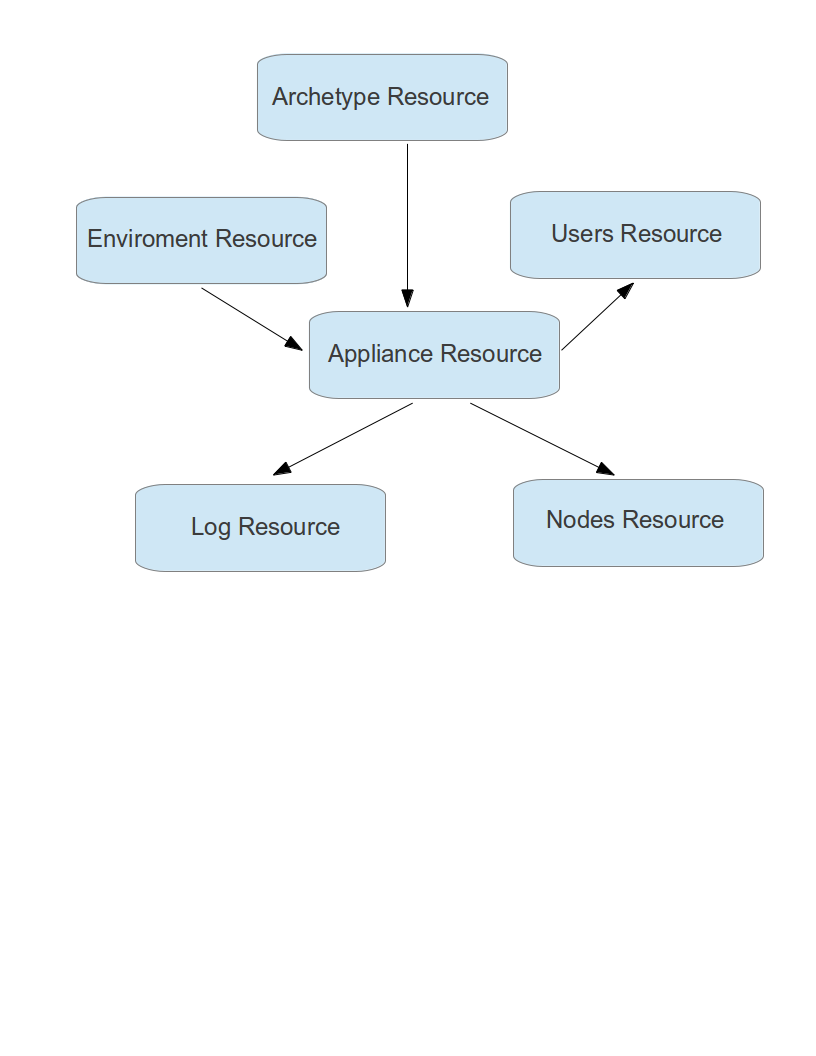
\includegraphics[scale=0.44]{fig/RelationshipsBetweenResources}
%  \caption{Visi'on de las relaciones entre recursos}
%  \label{fig:caption-bottom}
% \end{figure}

% El modelo de datos del Janu API esta basado en grupos de recursos, llamados colecciones:

% \begin{description}
% \item [Nodes collection] Un colecci'on de nodos consiste de todos los nodos que maneja el sistema. Es posible listar los nodos por pa'is o por ID.
% \item [Log collection] Una colecci'on de logs consiste en todos los logs recibidos de los appliance. Es posible listar los logs por appliance, fecha o por tipo de log.
% \item [Appliance collection] Una colecci'on de appliances consiste de todos los appliance registrados en el sistema. Es posible listarlos tambi'en por nodo o por ID.
% \item [Enviroment collection] Una colecci'on de enviroments consiste de todas los enviroments creados en el sistema. Es posible listarlos por un usuario especifico.
% \item [Archetype collection] Una colecci'on de arquetipos consiste en todos los arquetipos creados por los usuarios. Es posible listar los arquetipos por usuario, tipo o por ID.
% \item [User collection] Una colecci'on de usuarios consiste en todos los usuarios con registrados en el sistema. Es posible listarlos por ID o por su propio identificador.
% \end{description}

% \section{Provisioning API reference}
% El API esta organizado por tipo de recurso. Cada tipo de recurso tiene uno o mas representaciones de datos y uno o mas m'etodos.

% Muchos recursos de este API retornan  <code>application/json</code> y esperan el http header <code>Accept: application/json</code>. Si se omite o falla en pasar este header en la petici'on http, la petici'on fallara.

% \subsection{Nodes}

% \begin{table}[h]
% \scalebox{0.9}{
%   \begin{tabular}{|l |l |p{9.3cm} |}
%   \hline
%   \rowcolor{blueapi}
%     Method  & HTTP request & Description\\
%     \hline
%     list & GET /api/janu/nodes & Recibe una lista de recursos de nodos contenidos dentro del sistema.  \\
%     \hline
%     get & GET /api/janu/nodes/\{nodeId\} & Retorna el recurso de un nodo especifico.  \\
%     \hline
%     insert & POST /api/janu/nodes/\{nodeId\} & Crea un nuevo nodo en el sistema.  \\
%     \hline
%     update & PUT /api/janu/nodes/\{nodeId\} & Actualiza un nodo en el sistema.  \\
%     \hline
%     delete & DELETE /api/janu/nodes/\{nodeId\} & Elimina un nodo del sistema.  \\    
%     \hline
%   \end{tabular} 
%   }
% \caption[Nodes API]{Nodes API}
% \label{tab:nodesapi}
% \end{table}

% \subsection{Log}

% \begin{table}[h]
% \scalebox{0.9}{
%   \begin{tabular}{|l |l |p{8cm} |}
%   \hline
%   \rowcolor{blueapi}
%     Method  & HTTP request & Description\\
%     \hline
%     list & GET /api/janu/log/node/\{nodeId\} & Recibe una lista de recursos de log de un nodo especifico.  \\
%     \hline
%     list & GET /api/janu/log/appliance/\{applianceId\} & Recibe una lista de recursos de log de un appliance especifico.  \\
%     \hline
%   \end{tabular} 
%   }
% \caption[Log API]{Log API}
% \label{tab:logapi}
% \end{table}

% \newpage

% \subsection{Appliance}

% \begin{table}[h]
% \scalebox{0.9}{
%   \begin{tabular}{|l |p{9.7cm} |p{6cm} |}
%   \hline
%   \rowcolor{blueapi}
%     Method  & HTTP request & Description\\
%     \hline
%     get & GET /api/janu/appliance/\{applianceId\} & Recibe un recurso de un appliance especifico.  \\
%     \hline
%     insert & POST /api/janu/appliance/\{applianceId\} & Crea un nuevo appliance en el sistema.  \\
%     \hline
%     update & PUT /api/janu/appliance/\{applianceId\} & Actualiza un appliance en el sistema.  \\
%     \hline
%     delete & DELETE /api/janu/appliance/\{applianceId\} & Elimina un appliance del sistema.  \\   
%     \hline    
%     stop & POST /api/janu/appliance/\{applianceId\}/stop & Detiene un appliance del sistema.  \\   
%     \hline 
%     start & POST /api/janu/appliance/\{applianceId\}/start & Inicia un appliance del sistema.  \\   
%     \hline 
%     clone & POST /api/janu/appliance/\{applianceId\}/clone & Clona un appliance del sistema.  \\   
%     \hline    
%     move & POST /api/janu/appliance/\{applianceId\}/move/node/ \{nodeId\} & Mueve un appliance a un nodo especifico.  \\   
%     \hline   
%     restart & POST /api/janu/appliance/\{applianceId\}/restart & Reinicia un appliance.  \\   
%     \hline                 
%   \end{tabular} 
%   }
% \caption[Appliance API]{Appliance API}
% \label{tab:applianceapi}
% \end{table}

% \subsection{Enviroment}

% \begin{table}[h]
% \scalebox{0.9}{
%   \begin{tabular}{|l |p{9.7cm} |p{6cm} |}
%   \hline
%   \rowcolor{blueapi}
%     Method  & HTTP request & Description\\
%     \hline
%     get & GET /api/janu/enviroment/\{enviromentId\} & Recibe un recurso de un enviroment especifico.  \\
%     \hline
%     insert & POST /api/janu/enviroment/\{enviromentId\} & Crea un nuevo enviroment en el sistema.  \\
%     \hline
%     update & PUT /api/janu/enviroment/\{enviromentId\} & Actualiza un enviroment en el sistema.  \\
%     \hline
%     delete & DELETE /api/janu/enviroment/\{enviromentId\} & Elimina un enviroment del sistema.  \\   
%     \hline    
%   \end{tabular} 
%   }
% \caption[Enviroment API]{Enviroment API}
% \label{tab:enviromentapi}
% \end{table}

% \subsection{Archetype}

% \begin{table}[h]
% \scalebox{0.9}{
%   \begin{tabular}{|l |p{9.7cm} |p{6cm} |}
%   \hline
%   \rowcolor{blueapi}
%     Method  & HTTP request & Description\\
%     \hline
%     get & GET /api/janu/archetype/\{archetypeId\} & Recibe un recurso de un archetype especifico.  \\
%     \hline
%     insert & POST /api/janu/archetype/\{archetypeId\} & Crea un nuevo archetype en el sistema.  \\
%     \hline
%     update & PUT /api/janu/archetype/\{archetypeId\} & Actualiza un archetype en el sistema.  \\
%     \hline
%     delete & DELETE /api/janu/archetype/\{archetypeId\} & Elimina un archetype del sistema.  \\   
%     \hline    
%   \end{tabular} 
%   }
% \caption[Archetype API]{Archetype API}
% \label{tab:archetypeapi}
% \end{table}

% \newpage

% \subsection{User}

% \begin{table}[h]
% \scalebox{0.9}{
%   \begin{tabular}{|l |p{9.7cm} |p{6cm} |}
%   \hline
%   \rowcolor{blueapi}
%     Method  & HTTP request & Description\\
%     \hline
%     list & GET /api/janu/user/ & Recibe una lista de recursos de usuarios del sistema.  \\    
%     \hline
%     get & GET /api/janu/user/\{userId\} & Recibe un recurso de un usuario especifico.  \\
%     \hline
%     insert & POST /api/janu/user/\{userId\} & Crea un nuevo usuario en el sistema.  \\
%     \hline
%     update & PUT /api/janu/user/\{userId\} & Actualiza un usuario en el sistema.  \\
%     \hline
%     delete & DELETE /api/janu/user/\{userId\} & Elimina un usuario del sistema.  \\   
%     \hline    
%   \end{tabular} 
%   }
% \caption[User API]{User API}
% \label{tab:userapi}
% \end{table}

% \section{HTTP status codes}
% La API de aprovisionamiento intenta devolver c'odigos de estado HTTP apropiados para cada solicitud. La siguiente tabla describe los c'odigo HTTP significativos en el contexto del API de aprovisionamiento.

% \begin{table}[h]
% \scalebox{0.9}{
%   \begin{tabular}{|l |p{10.5cm}|}
%   \hline
%   \rowcolor{blueapi}
%     Code  & Explanation \\
%     \hline  
%     200 Ok & No error. \\
%     \hline
%     201 Created & Creation of a resource was successful. \\
%     \hline
%     304 Not modified & The resource hasn't changed since the time specified in the request's If-Modified-Since header. \\
%     \hline
%     400 Bad request & Invalid request URI or header, or unsupported nonstandard parameter. \\
%     \hline
%     401 Unauthorized & Authorization required. \\
%     \hline
%     403 Forbidden & Unsupported standard parameter, or authentication or authorization failed. \\
%     \hline
%     404 Not found & Resource (such as a feed or entry) not found. \\
%     \hline
%     405 Method Not Allowed & The specified method is not allowed against this resource. \\
%     \hline
%     409 Conflict & Specified version number doesn't match resource's latest version number. \\
%     \hline
%     500 Internal server error & Internal error. This is the default code that is used for all unrecognized server errors. \\
%     \hline   
%     501 Not Implemented & A header you provided implies functionality that is not implemented. \\
%     \hline
%   \end{tabular} 
%   }
% \caption[HTTP status codes]{HTTP status codes}
% \label{tab:httpstatuscodes}
% \end{table}

% \newpage

% \section{El estilo REST}
% REST es un estilo de arquitectura de software que proporciona un enfoque pr'actico y consistente para solicitar y modificar datos.

% El termino REST es la abreviatura para \"Representational State Transfer.\" En el contexto del Janu API, se refiere al uso de verbos HTTP para recibir y modificar representaciones de datos guardadas por el sistema de aprovisionamiento.

% En un sistema RESTful, los recursos se almacenan en un almac'en de datos, un usuario env'ia una solicitud al servidor para realizar una acci'on determinada (como la creaci'on, recuperaci'on, actualizaci'on o eliminaci'on de un recurso), y el servidor realiza la acci'on y env'ia una respuesta, a menudo en la forma de una representaci'on del recurso especificado.


% En API REST de Janu, el usuario especifica una acci'on con un verbo HTTP como POST, GET, PUT o DELETE. Especifica un recurso por un URI 'unico global de la siguiente forma:

% https://www.domain.edu.co/api/janu/resourcePath?parameters

% Debido a que todos los recursos del API tienen 'unica URI HTTP accesible, REST permite el almacenamiento en cach'e de datos y est'a optimizado para trabajar con una infraestructura distribuida de la web.

% \section{Formato de datos - JSON}
% JSON (JavaScript Object Notation) es un formato de datos com'un, independiente del lenguaje que proporciona una representaci'on de texto simple de estructuras de datos arbitrarias. Para obtener m'as informaci'on, ver json.org.

% \section{Ejemplos}
